\section{}
A frame of constant flexural rigidity $EI$ carries a concentrated load P at point E (Fig. \ref{fig:Q6ProblemDiagram}). 
Determine the reaction R at support A using Castigliano's theorem.

\begin{figure}[h]
    \centering
    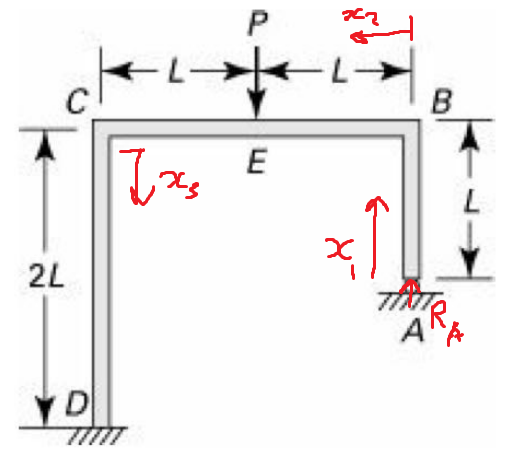
\includegraphics[width=0.5\linewidth]{Questions/Figures/Q6ProblemDiagram.png}
    \caption{Frame with pinned connection at A}
    \label{fig:Q6ProblemDiagram}
\end{figure}

The moment equation from A to B is:
\begin{align*}
    M_{AB} &= 0  \\
    \implies \frac{\partial M_{AB}}{\partial R_A} = 0 
\end{align*}

The moment equation from B to C is:
\begin{align*}
    M_{BC} &= R_A x - P \langle x - L \rangle^1, \quad \langle x - L \rangle^1 = (x-L)H\left(x - L\right)\\
    \implies \frac{\partial M_{BC}}{\partial R_A} &= x 
\end{align*}

The moment equation from C to D is:
\begin{align*}
    M_{CD} &= M_{BC}|_{x=2L} = 2LR_A - PL \\
    \implies \frac{\partial M_{CD}}{\partial R_A} &= 2L
\end{align*}

By Castigliano's theorem, the deflection at A is:
\begin{align*}
    \delta_A &= \frac{1}{EI} \left[\cancel{\int_{0}^{L} M_{AB} \left(\frac{\partial M_{AB}}{\partial R_A}\right) dx}
    + \int_{0}^{2L} M_{BC} \left(\frac{\partial M_{BC}}{\partial R_A}\right) dx 
    + \int_{0}^{2L} M_{CD} \left(\frac{\partial M_{CD}}{\partial R_A}\right) dx \right] \\
    &= \frac{1}{EI} \left[\int_{0}^{L} R_A x^2 dx + \int_{L}^{2L} R_A x^2 - Px(x-L) dx 
    + \int_{0}^{2L} (2LR_A - PL)(2L) dx \right] \\
    &= \frac{1}{EI} \left[\frac{L^3R_A}{3} - \frac{4L^3(P-2R_A)}{3} - \frac{L^3(5P-14R_A)}{6} \right] 
\end{align*} 

Since the pin at A cannot carry deflection, $\delta_A = 0$. Therefore,
\begin{align*}
    \delta_A \overset{\text{set}}{=} 0 &= \frac{1}{EI} \left[\frac{L^3R_A}{3} - \frac{4L^3(P-2R_A)}{3} - \frac{L^3(5P-14R_A)}{6} \right] \\
    \implies R_A &= \boxed{\frac{29P}{64}}
\end{align*}


